% !TeX spellcheck = da_DK
\documentclass[11pt, fleqn]{article}
%\usepackage{siunitx}
\usepackage{texfiles/SpeedyGonzales}
\usepackage{texfiles/MediocreMike}
\title{02466 Project work in Artificial Intelligence and Data LOGBOOK}
\author{Oskar Eiler Wiese Christensen s183917, Anders Henriksen s183904, Dagh}

\begin{document}
	\maketitle
		
\section*{Project Meetings}
	
	%Questions \\
	%Reading, who and what \\
	%Implementation, who and what \\
	%Results, who and what \\
	%Decisions, who and what, what do you do alone, what do you do together
	
	\textbf{Week 08:}  19.02.2020 \\\\
	\noindent
	Hvilke bias eksisterer i dataen? \\ 
	\begin{figure}[H]
		\centering
		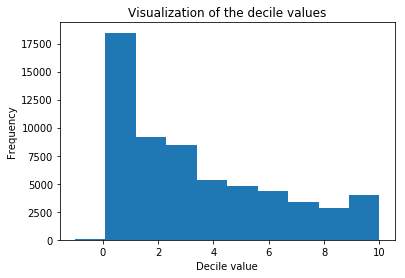
\includegraphics[width=0.3\linewidth]{billeder/decil.png}
	\end{figure}

	\begin{figure}[H]
		\centering
		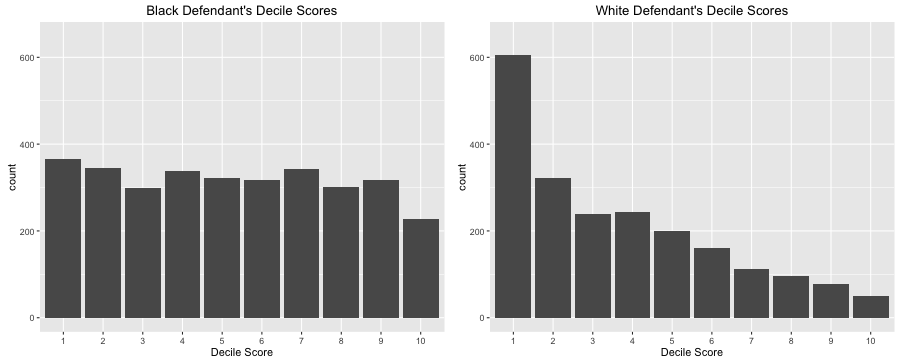
\includegraphics[width=0.7\linewidth]{billeder/black_white}
	\end{figure}
	\noindent
	There exists a recial bias in the dataset, which is indicated by the histograms above. 
	
\section*{Supervisor Meetings}
	
	\textbf{Week 07:}  12.02.2020 \\\\
	\noindent
%	Presentation of results since last meeting \\
	Meeting notes: \\ Fællesmøder samt personlige møde. (Hver anden uge er individuele). \\0. Vi får et datasæt (COMPASS) - ligger online \\
	1. Hvordan er dataen skæv? (Hvilke bias eksisterer i dataen) (Hvordan finder man helt præcist ud af det?) (Hvad betyder det at der er en bias?) \\
	2. Hvad gør skæv data ved min algoritme? (hvad betyder bias i en algoritme) (Hvordan kvantificeres/verificeres bias i algorimten?) \\
	3. Equality of Opportunity in Supervised Learning (forstå, implementer og valider) \\ 
	4. Etisk diskussion (Sune Filosof)
	\\\\\\\\
	\textbf{Week 08:}  19.02.2020 \\\\
	\noindent
	%	Presentation of results since last meeting \\
	Meeting notes: \\ Feature extraction
	\\\\
	Action points for next week: N/A
	\\\\\\\\
	\textbf{Week 09:}  26.02.2020 \\\\
	\noindent
	%	Presentation of results since last meeting \\
	Meeting notes: 
	\\\\
	Action points for next week
	\begin{itemize}
		\item  
	\end{itemize}

\section*{Definition af Bias:}
	
	Bias i datasæt 
		
	
\end{document}
